\chapter{ПОСТАНОВКА ЗАДАЧИ ПОЛУЧЕНИЯ, АНАЛИЗА И ОБРАБОТКИ ЭКСПЕРТНОЙ ИНФОРМАЦИИ} \label{chapt1}

\section{Возникновение области} \label{sect1_1}
В настоящее время в области IT набрало большую популярность системы удаленной поддержки информационной инфраструктуры, так называемый «Аутсорсинг». Ввиду развития рынка компаниям становится невыгодно держать свой штат службы поддержки, и они отдают свою инфраструктуру сторонней компании.
Большинство проблем, которые решает удаленная служба поддержки носят весьма тривиальный характер :
\begin{itemize}
	\item Установить приложение
	\item Переустановить приложение
	\item Решить проблему с доступом к тому или иному ресурсу
\end{itemize}
Данные проблемы решают специалисты технической поддержки. Обычно техническая поддержка делится на несколько линий:
\begin{enumerate}
	\item Первая линия. Решение уже известных, задокументированных проблем, работа напрямую с пользователем
	\item Вторая линия. Решение ранее неизвестных проблем
	\item Третья линия. Решение сложных и нетривиальных проблем
	\item Четвертая линия. Решение архитектурных проблем инфраструктуры
\end{enumerate}

Каждая линия поддержки представлена специалистами. В среднем команда, обслуживающая одного заказчика насчитывает 60 человек. Процентное соотношение специалистов разных линий поддержки отображено на Диаграмме \ref{img:ITSMTeamComposition}

\begin{figure} [h] 
  \center
  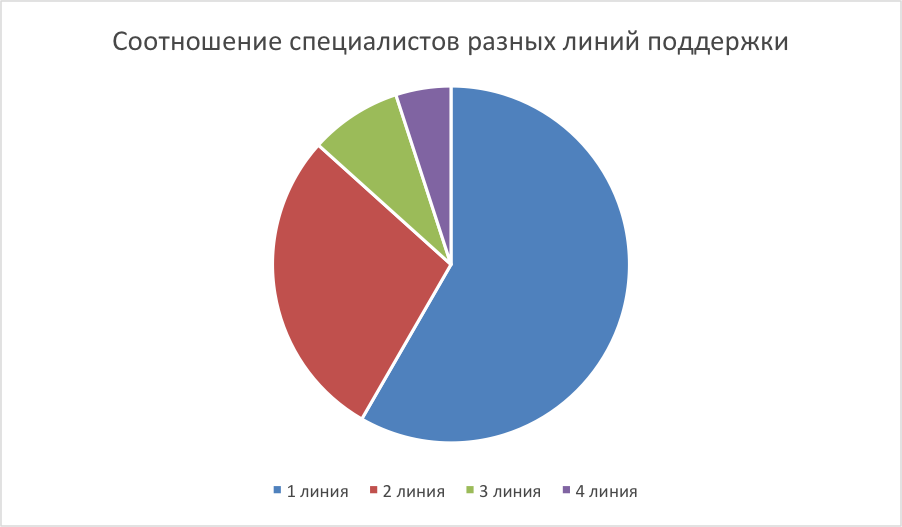
\includegraphics [scale=0.7] {ITSMTeamComposition}
  \caption{Диаграмма состава команд} 
  \label{img:ITSMTeamComposition}  
\end{figure}

Работа специалиста 1 линии поддержки состоит из множества рутинных и простых задач. На Диаграмме \ref{img:EngineerTasks}  показано соотношение разных типов проблем, встречающихся во время работы поддержки

\begin{figure} [h] 
  \center
  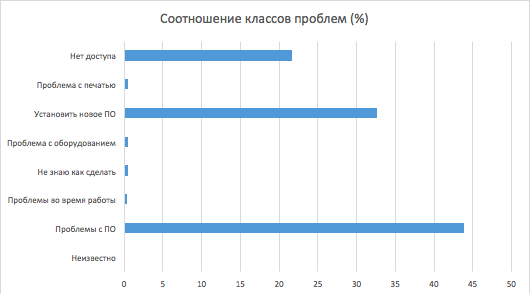
\includegraphics [scale=0.7] {EngineerTasks}
  \caption{Диаграмма соотношений типов проблем} 
  \label{img:EngineerTasks}  
\end{figure}

\begin{table} [htbp]
  \centering
  \parbox{15cm}{\caption{Категории инцидентов}\label{IncidentDescription}}
%  \begin{center}
  \begin{tabular}{| p{7cm} || p{7cm} |}
  \hline
  \hline
Категория & Описание \\
  \hline
Проблема с ПО	& Проблема при запуске ПО на компьютере. Решается переустановкой \\
Проблемы во время работы  & Проблема с функционированием программного обеспечения\\
Как сделать & Запрос на инструкцию по работе с тем или иным компонентом рабочей станции \\
Проблема с оборудованием  & Неполадки на уровне оборудования \\
Установить новое ПО       & Требование установки нового программного обеспечения \\
Проблема с печатью        & Установка принтера в систему \\
Нет доступа               & Нет доступа к общим ресурсам \\
  \hline
  \hline
  \end{tabular}
%  \end{center}
\end{table}

Решение части задач может быть автоматизировано, а специалисты получат дополнительное время на решение более интересных задач. 
Проблема заключается в автоматизации решения рутинных задач в области удаленной поддержки инфраструктуры.

%\newpage
%============================================================================================================================

\section{Прогноз развития области} \label{sect1_2}
Основной тенденцией в развитии области удаленной поддержки инфраструктуры является попытки удешевить и улучшить стоимость предоставления услуг. \\
Компании, работающие на этом рынке вкладывают большие деньги в автоматизацию. Кроме того современное развитие науки и техники, а точнее вычислительных мощностей позволяет автоматизацию даже самых наукоемких процессов. \\
Дальнейшим развитием области является замена человеческих специалистов на автоматические системы. Многие ведущие компании ведут разработки в этом направлении. Например, компания HP. Данная компания имеет свою системы по регистрации подобных инцидентов и сейчас ведется работа над автоматизацией системы. \\

\section{Методологии, используемые в области IT аутсорсинга: ITIL и ITSM} \label{sect1_3}
В области IT аутсорсинга есть несколько готовых стандартов ведения работ. Одним из таких стандартов является библиотека ITIL. Данные стандарт описывает лучшие практики организации работ в области IT аутсорсинга. Используемый в библиотеки подход соответствует стандартам ISO 9000 (ГОСТ Р ИСО 9000) .
Наличие стандартов в области диктует унифицированность постановки проблем, а также унифицированность алгоритмов решения. Такие предпосылки говорят о возможности частично или в некоторых случаях полной автоматизации решения проблем.
\section{Постановка задачи} \label{sect1_4}
Задачами данного исследования являются:
\begin{itemize}
	\item Изучение возможности автоматизации области удаленной поддержки инфраструктуры путем анализа области
	\item Выработка критериев и сравнительный анализ существующих решений в области
	\item Создание программного комплекса (фреймворка) для автоматизации поддержки удаленной инфраструктуры
	\item Подсчет статистических результатов работы комплекса
\end{itemize}




%\newpage
%============================================================================================================================

\section{Формулы} \label{sect1_3}

Благодаря пакету \textit{icomma}, \LaTeX~одинаково хорошо воспринимает в качестве десятичного разделителя и запятую ($3,1415$), и точку ($3.1415$).

\subsection{Ненумерованные одиночные формулы} \label{subsect1_3_1}

Вот так может выглядеть формула, которую необходимо вставить в строку по тексту: $x \approx \sin x$ при $x \to 0$.

А вот так выглядит ненумерованая отдельностоящая формула c подстрочными и надстрочными индексами:
$$
(x_1+x_2)^2 = x_1^2 + 2 x_1 x_2 + x_2^2
$$

При использовании дробей формулы могут получаться очень высокие:
$$
  \frac{1}{\sqrt(2)+
  \displaystyle\frac{1}{\sqrt{2}+
  \displaystyle\frac{1}{\sqrt{2}+\cdots}}}
$$

В формулах можно использовать греческие буквы:
$$
\alpha\beta\gamma\delta\epsilon\varepsilon\zeta\eta\theta\vartheta\iota\kappa\lambda\\mu\nu\xi\pi\varpi\rho\varrho\sigma\varsigma\tau\upsilon\phi\varphi\chi\psi\omega\Gamma\Delta\Theta\Lambda\Xi\Pi\Sigma\Upsilon\Phi\Psi\Omega
$$

%\newpage
%============================================================================================================================

\subsection{Ненумерованные многострочные формулы} \label{subsect1_3_2}

Вот так можно написать две формулы, не нумеруя их, чтобы знаки равно были строго друг под другом:
\begin{eqnarray}
  f_W & = & \min \left( 1, \max \left( 0, \frac{W_{soil} / W_{max}}{W_{crit}} \right)  \right), \nonumber \\
  f_T & = & \min \left( 1, \max \left( 0, \frac{T_s / T_{melt}}{T_{crit}} \right)  \right), \nonumber
\end{eqnarray}

Можно использовать разные математические алфавиты:
\begin{eqnarray}
\mathcal{ABCDEFGHIJKLMNOPQRSTUVWXYZ} \nonumber \\
\mathfrak{ABCDEFGHIJKLMNOPQRSTUVWXYZ} \nonumber \\
\mathbb{ABCDEFGHIJKLMNOPQRSTUVWXYZ} \nonumber
\end{eqnarray}

Посмотрим на систему уравнений на примере аттрактора Лоренца:

$$
\left\{
  \begin{array}{rl}
    \dot x = & \sigma (y-x) \\
    \dot y = & x (r - z) - y \\
    \dot z = & xy - bz
  \end{array}
\right.
$$

А для вёрстки матриц удобно использовать многоточия:
$$
\left(
  \begin{array}{ccc}
  	a_{11} & \ldots & a_{1n} \\
  	\vdots & \ddots & \vdots \\
  	a_{n1} & \ldots & a_{nn} \\
  \end{array}
\right)
$$


%\newpage
%============================================================================================================================
\subsection{Нумерованные формулы} \label{subsect1_3_3}

А вот так пишется нумерованая формула:
\begin{equation}
  \label{eq:equation1}
  e = \lim_{n \to \infty} \left( 1+\frac{1}{n} \right) ^n
\end{equation}

Нумерованых формул может быть несколько:
\begin{equation}
  \label{eq:equation2}
  \lim_{n \to \infty} \sum_{k=1}^n \frac{1}{k^2} = \frac{\pi^2}{6}
\end{equation}

В последствии на формулы (\ref{eq:equation1}) и (\ref{eq:equation2}) можно ссылаться.

%\newpage
%============================================================================================================================

\clearpage
